\chapter {Berlin Institute for Software Defined Networks} \label{chap:bisdn} %% chapter 3

\section {Introduction}

\begin{figure} [!htbp]
    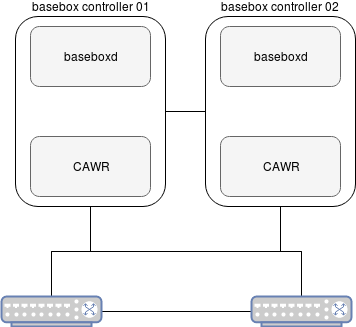
\includegraphics[width=.4\textwidth]{bisdn/basebox}
    \caption{Basebox architecture}
\end{figure}

As the SDN market grows larger and larger in the networking world, new applications and products are developed and improved. Seeing the prevalence of closed source and proprietary solutions for this market, a need for open
products that enable further growth and innovation in cloud DCNs is evident. The main gain in moving from vertically integrated solutions, is the decrease of costs involved, as cheaper solutions can be found in whitebox 
\footnote {whitebox switches are} switches and open sourced networking applications. With this motivation, BISDN developed Basebox, a Linux-powered solution to integrate switches and SDN controllers, allowing for data center 
operators to configure and manage networks using linux commands, removing the need for having to manage several devices with different interfaces and workflows, and adding the capability of running standard networking applications 
on top of the controllers and switches. Basebox also includes the possiblity of running in a failover scenario, by introducing a backup controller for the network, and the possibility of creating a giant switch abstraction, 
by adding another controller, CAWR, and having this manage all the southbound switches.

\par In this chapter we focus on this product, on the first two sections some characteristics of the developed product are described, then we focus on the development of a management API, presenting the required technologies that 
were implemented, and then finally display the results that were obtained in this part of the thesis.

\section {Existing product}

\subsection {baseboxd}
\subsection {CAWR}

\section {Management API}

Due to the capabilities of Basebox of being a SDN controller used in data centers and a mission critical component for the network operators, it needed management capabilities, so that managing and operating infrastructure becomes 
an easier task. As such, the original problem presented was to build an interface extending the original work, so that the network statistics and the information of the topology could be easily displayed. There were several steps
then necessary to understand the problem, and be able to choose the best approach to this problem. The requirements for the proposed system were:

\begin {itemize}
    \item Display the topology information reported by CAWR, including the internal switch links, and the LACP discovered bond interfaces on the servers
    \item Display the port and link statistics for both switches
    \item Design an alerting system, so that network operators can be informed of changes on the network state
    \item Provide some diagnostic capabilities
\end {itemize}

\par The development of the work was the divided on two parts: the first part would be to implement the API needed to export the port statistics from baseboxd and CAWR, including a Graphical User Interface (GUI); and the second 
part was to study the alerting system, that would look into the statistics provided by the controllers, and design some rules so that QoS rules could be applied in the final product. This section describes the technologies needed 
to implement the API for Basebox.

\subsection {Data models}

Data models are abstract concepts that map the properties of entities and organizes their data, also defining how they relate to each other. To create a switch management interface, the entities we want to model are then 
the switches themselves, with attributes like the switch name, and the port counters, and the relationships of the data will allow us to display the links and topology of the network. One of the considerations that were taken into 
account when choosing the data models was the compatibility with standardized data models by the organizational entities like the IETF and the OpenConfig. 
\par The \textit{ NETCONF } network configuration model, which we explore further in \ref{ssec:grpc} also defines a data modelling language known as \textit{ YANG }, which is used in this protocol to model its configuration and data,
and the remote procedure calls \cite { CITE - rfc 6020 }. By utilizing models defined in this language, the following condition is met: since this is a specific language for configuration and monitoring of networking 
devices, the existing data models will be similar to the ones that should be employed in the development of the management API.



\subsection {Protocols}

\subsubsection {NETCONF}
\subsubsection {gRPC} \label {ssec:grpc}
\subsubsection {GUI}

\section {Results}
